\documentclass[UTF8,a4paper,11pt,fontset=fandol]{ctexart}
\usepackage{geometry}
\geometry{margin=2.2cm}
\usepackage{amsmath,amssymb,longtable,booktabs,array,hyperref,xcolor,enumitem,graphicx,float}
\hypersetup{colorlinks=true,linkcolor=blue,urlcolor=blue}
\setlist[itemize]{leftmargin=1.3em,itemsep=0.2em}
\definecolor{notegray}{RGB}{246,248,251}
\title{P09. Overtaking-enabled Eco-approach Control at Signalized Intersections for Connected and Automated Vehicles\\中英双语博士精读笔记}
\author{Haoxuan Dong; Weichao Zhuang; Guoyuan Wu; Zhaojian Li; Guodong Yin; Ziyou Song}
\date{2023 · arXiv preprint}
\begin{document}
\maketitle

\noindent\textbf{Theme / 主题：} Eco-approach + relaxed FIFO\\
\textbf{Method family / 方法族：} Overtaking-enabled two-stage eco-approach / 允许超车的两阶段生态接近控制\\
\textbf{PDF pages / 页数：} 12 \quad
\textbf{Relevance / 相关度：} 84/100\\
\textbf{Source / 来源：} \url{https://arxiv.org/abs/2306.09736}

\section{论文全景速览与核心贡献 / High-Level Overview \& Core Contributions}
\subsection{研究背景与痛点 / Background \& Pain Points}
这篇论文位于“Eco-approach + relaxed FIFO”方向。对你的 JSSP-based Intersection Management 课题，它回答的是高层调度、低层轨迹平滑、安全过滤或真实验证中的一个关键子问题：如何让车辆在路口少停、少冲突、少能耗，同时保持在线可执行。

The paper belongs to the theme of Eco-approach + relaxed FIFO. For a JSSP-based intersection-management thesis, it illuminates one of the key layers: scheduling, smoothing, safety filtering, or real-world validation.

\textbf{Pain point / 痛点：} Signalized intersection and overtaking/lane planning assumptions are outside the current fixed-route JSSP scope.

\subsection{核心科学问题 / Core Scientific Question}
在信号交叉口中，放松 FIFO 队列并允许超车，能否同时降低能耗和延误？

Can relaxing FIFO with overtaking-enabled lane optimization reduce both energy use and delay at signalized intersections?

\subsection{科学贡献 / Scientific Contributions}
\begin{itemize}
\item 方法贡献 (method contribution)：Receding-horizon two-stage control: dynamic-programming lane optimization followed by PMP speed trajectory optimization.
\item 安全/避碰贡献 (safety contribution)：Handles dynamic disturbance from preceding vehicles and lane-choice constraints.
\item 平滑/停止避免贡献 (smoothing contribution)：Relaxes FIFO queuing at signalized intersections to reduce driving cost, energy consumption, and delay.
\item 创新力度评判 (reviewer judgement)：较强工程洞察：明确挑战 FIFO 保守性，对 JSSP 重排序动机非常有用。
\end{itemize}


\subsection{核心概念对照 / Core Concepts}
\begin{longtable}{p{0.24\linewidth}p{0.28\linewidth}p{0.40\linewidth}}
\toprule
中文概念 & English Concept & Role / 学术作用\\
\midrule
自动交叉口管理 & Autonomous Intersection Management & 把信号控制替换为车辆级调度与控制。 \\
轨迹平滑 & Trajectory Smoothing & 减少急加减速、停车和能耗峰值。 \\
安全约束 & Safety Constraints & 把碰撞风险写成距离、时间间隔或屏障函数。 \\
Overtaking-enabled two-stage eco-approach & 允许超车的两阶段生态接近控制 & 该论文的核心方法族。 \\
\bottomrule
\end{longtable}

\section{教材式学习路径与关键截图 / Textbook-Style Study Path \& PDF Snapshots}
\subsection{学习路径 / Study Path}
\begin{itemize}
\item 第一遍先读首页截图、摘要与引言，确认研究问题和场景假设。
\item 第二遍沿着技术路线图复现模型变量、约束和求解器输入输出。
\item 第三遍逐节阅读 section deep reading，对照 PDF 截图检查公式、图表和实验。
\item 第四遍只站在审稿人视角重读实验，判断 baseline、公平性、消融和鲁棒性。
\item 最后把博士 checklist 写成自己的复现实验或论文拓展计划。
\end{itemize}


\subsection{博士阅读 Checklist / Doctoral Reading Checklist}
\begin{itemize}
\item 能否独立重写核心公式：车道 DP 与速度 PMP 的两阶段目标 / Two-stage lane-DP and speed-PMP objective，并解释每个符号的物理意义？
\item 能否画出输入-模型-算法-控制-验证的数据流图？
\item 能否指出至少两个强假设，并说明它们在真实交通中何时失效？
\item 能否复述实验基准是否公平，指标是否覆盖效率、安全、能耗和计算时间？
\item 能否提出一个与自己 JSSP/RL/smoother 课题直接相连的拓展实验？
\end{itemize}


\subsection{关键截图讲解 / PDF Snapshot Explanation}
Screenshots are selected anchors from the local PDFs for study and parallel reading. They do not replace the original paper.

\begin{figure}[H]
\centering

\includegraphics[width=0.92\linewidth]{../../assets/P09_dong2023overtaking/01_title_and_abstract_p1.jpg}
\caption{首页与摘要 / Title and abstract page (p.1, full\_page). 这张截图用于把笔记中的抽象概念拉回原论文页面，便于你平行阅读原文、公式、图表和实验设置。 与当前课题的连接：Supports the critique that FCFS/FIFO can be suboptimal and that speed smoothing should be coupled to sequencing.}
\end{figure}

\begin{figure}[H]
\centering
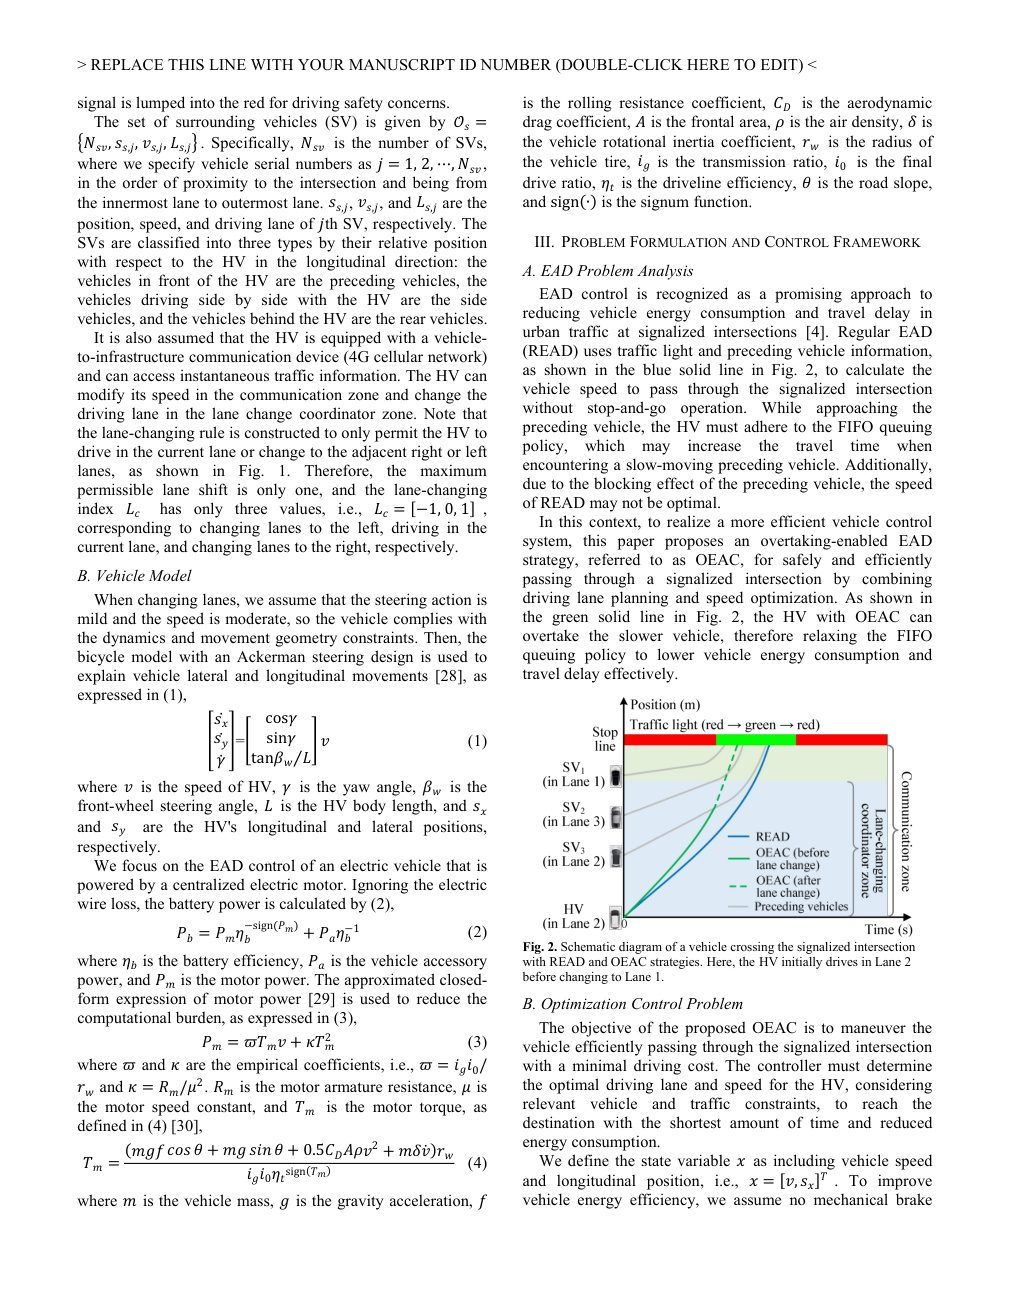
\includegraphics[width=0.92\linewidth]{../../assets/P09_dong2023overtaking/02_modeling_or_problem_setup_p3.jpg}
\caption{建模或问题设定页 / Modeling or problem-setup page (p.3, full\_page). 这张截图用于把笔记中的抽象概念拉回原论文页面，便于你平行阅读原文、公式、图表和实验设置。 与当前课题的连接：Supports the critique that FCFS/FIFO can be suboptimal and that speed smoothing should be coupled to sequencing.}
\end{figure}

\begin{figure}[H]
\centering
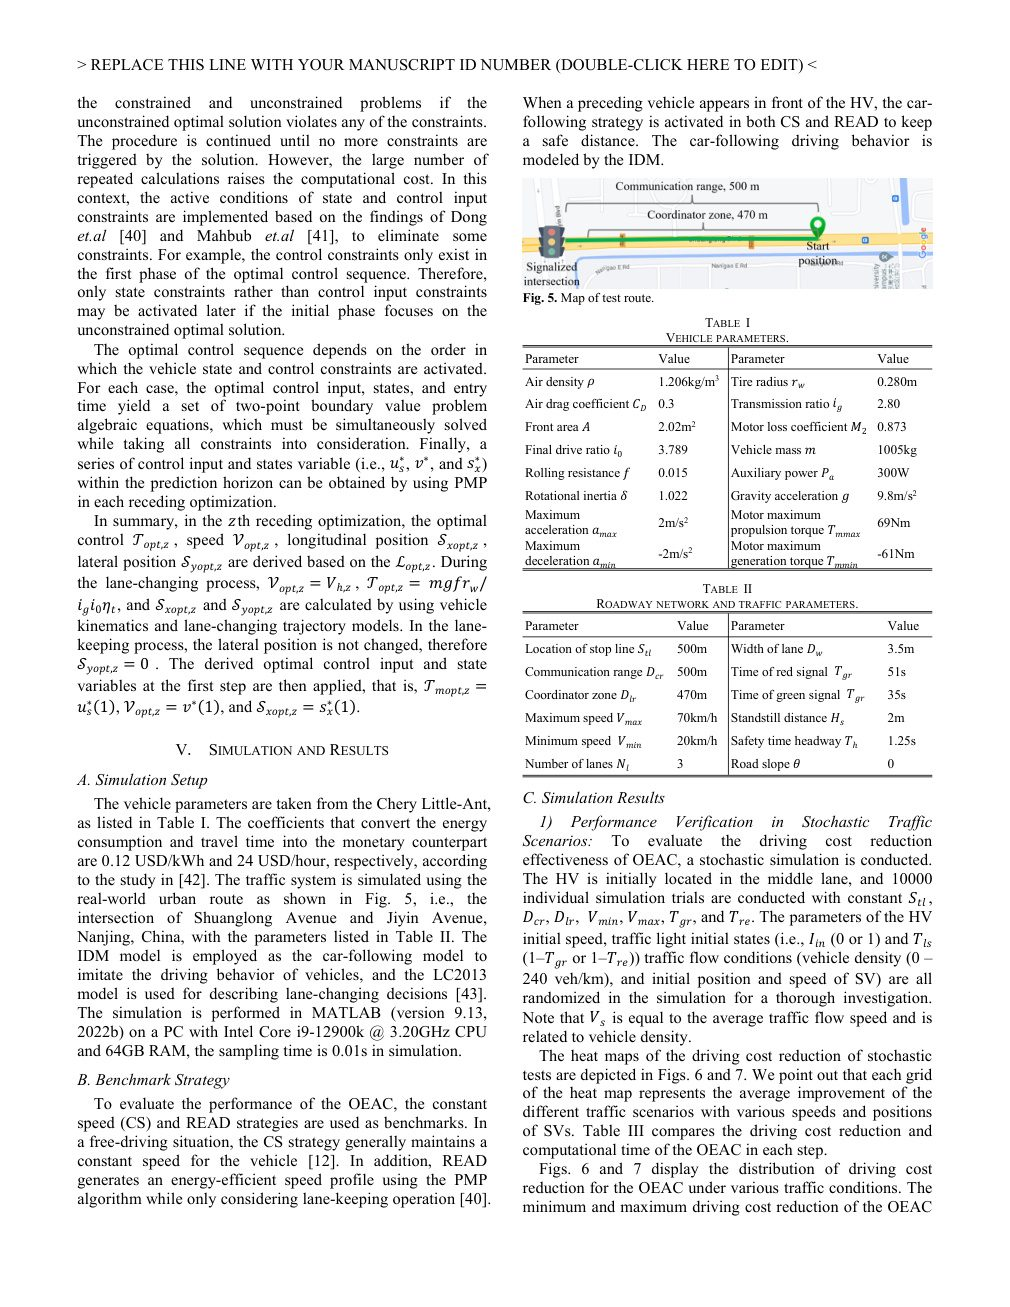
\includegraphics[width=0.92\linewidth]{../../assets/P09_dong2023overtaking/03_experiments_or_results_p8.jpg}
\caption{实验或结果页 / Experiments or results page (p.8, full\_page). 这张截图用于把笔记中的抽象概念拉回原论文页面，便于你平行阅读原文、公式、图表和实验设置。 与当前课题的连接：Supports the critique that FCFS/FIFO can be suboptimal and that speed smoothing should be coupled to sequencing.}
\end{figure}

\begin{figure}[H]
\centering
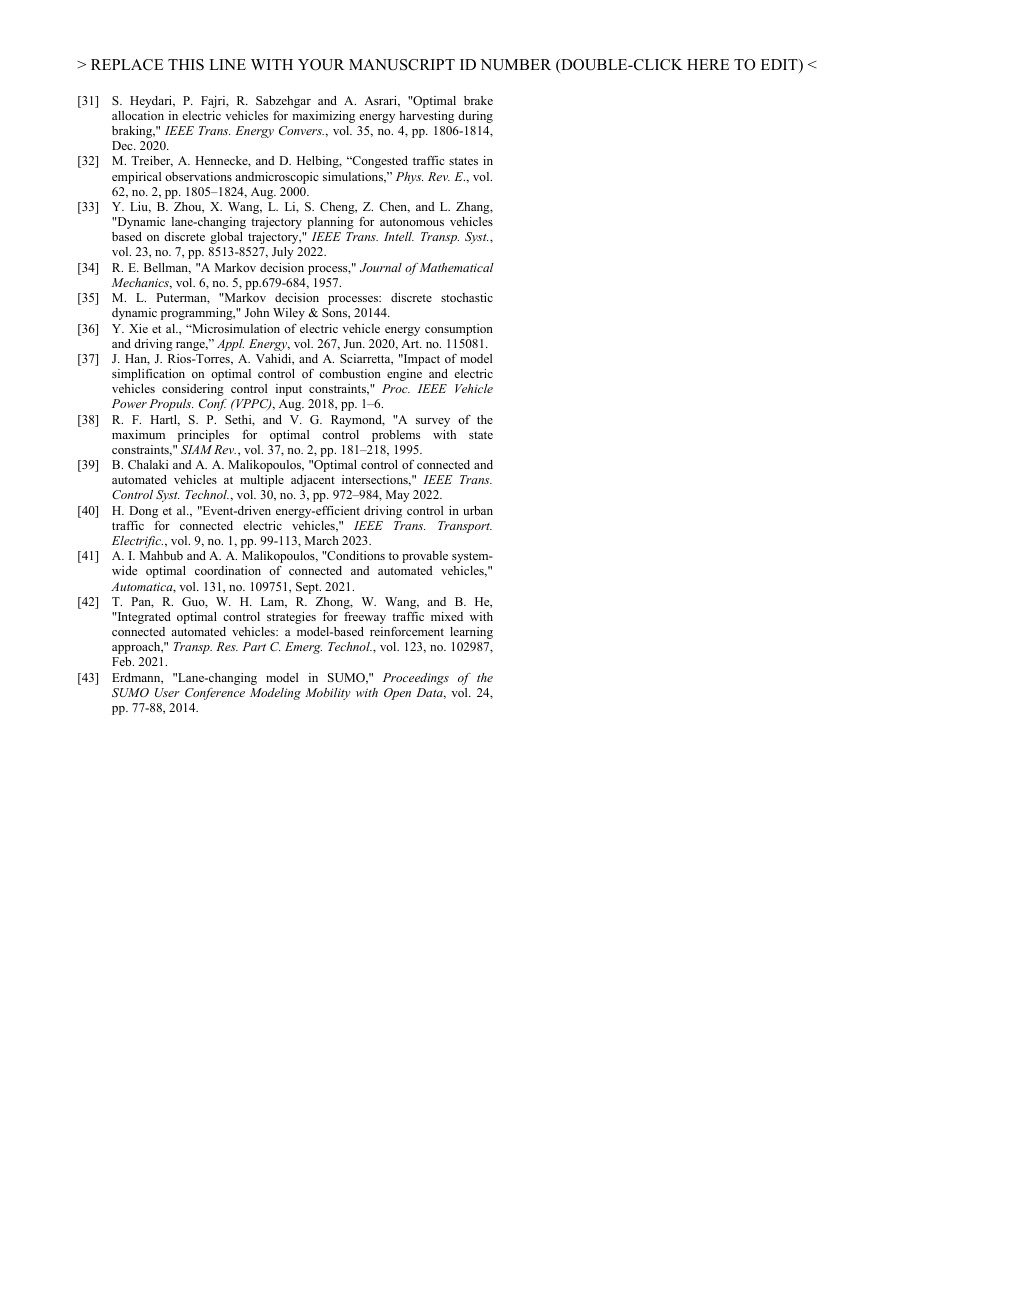
\includegraphics[width=0.92\linewidth]{../../assets/P09_dong2023overtaking/04_conclusion_or_limitations_p12.jpg}
\caption{结论或局限页 / Conclusion or limitations page (p.12, full\_page). 这张截图用于把笔记中的抽象概念拉回原论文页面，便于你平行阅读原文、公式、图表和实验设置。 与当前课题的连接：Supports the critique that FCFS/FIFO can be suboptimal and that speed smoothing should be coupled to sequencing.}
\end{figure}

\begin{figure}[H]
\centering

\includegraphics[width=0.92\linewidth]{../../assets/P09_dong2023overtaking/05_supplemental_reading_page_p2.jpg}
\caption{补充精读页 / Supplemental close-reading page (p.2, full\_page). 这张截图用于把笔记中的抽象概念拉回原论文页面，便于你平行阅读原文、公式、图表和实验设置。 与当前课题的连接：Supports the critique that FCFS/FIFO can be suboptimal and that speed smoothing should be coupled to sequencing.}
\end{figure}


\section{章节精读与逐段导读 / Section-by-Section Deep Reading \& Walkthrough}
\subsection*{p.1 I. INTRODUCTION}
\textbf{章节目标 / Learning goal：} 建立研究动机：为什么传统信号控制、FCFS 或单车控制不足以处理该论文关注的交叉口协同问题。

Understand why the paper needs a new coordination method rather than a standard signal, FCFS, or single-vehicle controller.

\textbf{关键论点 / Key argument：} 这一部分通常把痛点落到 Eco-approach + relaxed FIFO：既要提高效率，又要保持安全与在线可执行。

\textbf{技术焦点 / Technical focus：} 精读时标出作者批判的 baseline、场景假设、交通参与者类型和隐含优化目标。

\textbf{审稿追问 / Reviewer question：} 作者指出的痛点是否真的需要新方法，还是可以由更强的优化器/更保守规则解决？

\subsection*{p.2 II. INTERSECTIONCROSSINGSCENARIO AND}
\textbf{章节目标 / Learning goal：} 承接前后章节，补充局部定义、案例或实现细节。

Recover implementation details needed for reproduction.

\textbf{关键论点 / Key argument：} 这类章节常常不是主贡献，但决定你能否真正复现方法。

\textbf{技术焦点 / Technical focus：} 检查它是否给出了参数、伪代码、场景划分或实现细节。

\textbf{审稿追问 / Reviewer question：} 跳过该节会不会导致公式或实验无法复现？

\subsection*{p.3 III. PROBLEMFORMULATION ANDCONTROLFRAMEWORK}
\textbf{章节目标 / Learning goal：} 把自然语言交通问题压缩为变量、状态、约束、目标函数或图结构。

Translate the traffic problem into variables, states, constraints, objectives, or graph relations.

\textbf{关键论点 / Key argument：} 本节是复现论文的核心入口，应与公式“车道 DP 与速度 PMP 的两阶段目标 / Two-stage lane-DP and speed-PMP objective”一起读。

\textbf{技术焦点 / Technical focus：} 逐项检查车辆状态、冲突关系、控制输入、时间/空间索引和安全阈值是否定义完整。

\textbf{审稿追问 / Reviewer question：} 这些建模假设在混合交通、通信延迟、感知误差和高密度车流下是否仍成立？

\subsection*{p.4 IV. OVERTAKING-ENABLEDECO-APPROACH}
\textbf{章节目标 / Learning goal：} 解释算法如何把模型转化为可执行决策，并说明在线运行机制。

Trace how the paper turns the model into executable online decisions.

\textbf{关键论点 / Key argument：} 第一阶段用动态规划选择车道和超车策略，打破传统 FIFO；第二阶段用 PMP/最优控制生成速度曲线。滚动时域使策略能对前车扰动重新规划。

\textbf{技术焦点 / Technical focus：} 画出输入、核心求解器、输出和安全检查接口，明确哪些步骤是优化、哪些是规则、哪些是学习。

\textbf{审稿追问 / Reviewer question：} 若算法某一步失败，论文有没有 fallback、重规划或安全过滤机制？

\subsection*{p.8 V. SIMULATION ANDRESULTS}
\textbf{章节目标 / Learning goal：} 验证方法是否在公平基准下改善效率、安全、能耗或计算时间。

Check whether the claimed improvements are supported by fair baselines and meaningful metrics.

\textbf{关键论点 / Key argument：} 实验应与论文声称的贡献闭环：Extensive simulations report average driving-cost improvements over constant-speed and regular eco-approach baselines.

\textbf{技术焦点 / Technical focus：} 重点追踪指标：驾驶成本、能耗、延误、停车次数、超车次数和计算耗时。 同时检查仿真平台、交通需求和随机性设置。

\textbf{审稿追问 / Reviewer question：} 实验是否只展示平均收益，还是覆盖了高密度、异常扰动和失败案例？


\subsection{逐段式导读 / Paragraph-Level Walkthrough}
\paragraph{Opening motivation / 开篇动机段}先把作者的痛点翻译成一句博士问题：在信号交叉口中，放松 FIFO 队列并允许超车，能否同时降低能耗和延误？ 读这一段时不要急着接受动机，要追问传统 FCFS、信号灯或保守 MPC 为什么不足。

Turn the opening motivation into one doctoral-level question and test whether the paper truly needs a new method.

\paragraph{Assumption and setting / 假设与场景段}把车辆类型、通信条件、路口类型和动力学假设列成表。该文的关键边界包括：车辆具备安全超车和变道能力。；信号相位和前车扰动可预测。；车道变化不会引入未建模的横向风险。

List vehicle type, communication, intersection setting, and dynamics assumptions before reading the equations.

\paragraph{Model and notation / 模型与符号段}围绕核心公式“车道 DP 与速度 PMP 的两阶段目标 / Two-stage lane-DP and speed-PMP objective”复写符号表，确认每个变量是决策变量、状态变量、参数还是约束阈值。

Rewrite the symbol table around the core formulation and classify variables as states, decisions, parameters, or constraints.

\paragraph{Algorithm mechanism / 算法机制段}把算法读成一条数据流：输入交通状态，执行 Receding-horizon two-stage control: dynamic-programming lane optimization followed by PMP speed trajectory optimization.，输出可执行通行/控制决策，并检查安全接口。

Read the algorithm as a dataflow from traffic state to executable sequence/control decision, with explicit safety interfaces.

\paragraph{Experiment and evidence / 实验证据段}不要只看作者报告的提升，要检查基准、公平性和指标。本文验证描述为：Extensive simulations report average driving-cost improvements over constant-speed and regular eco-approach baselines.

Go beyond reported gains and inspect baselines, fairness, metrics, and computation time.

\paragraph{Reviewer synthesis / 审稿式总结段}最后把贡献拆成可发表与需补强两部分。对你课题最直接的用途是：Supports the critique that FCFS/FIFO can be suboptimal and that speed smoothing should be coupled to sequencing.

Separate publishable contribution from missing evidence, then connect the result to your own thesis architecture.


\section{技术路线图与贡献量评估 / Technical Route \& Contribution Matrix}
\begin{longtable}{p{0.08\linewidth}p{0.24\linewidth}p{0.58\linewidth}}
\toprule
Step & Stage / 阶段 & Content / 内容\\
\midrule
1 & 输入 / Input & 车辆状态、路径/车道、交通需求、信号或协同信息。 \\
2 & 建模 / Modeling & 车道 DP 与速度 PMP 的两阶段目标 / Two-stage lane-DP and speed-PMP objective \\
3 & 核心求解 / Core solver & Receding-horizon two-stage control: dynamic-programming lane optimization followed by PMP speed trajectory optimization. \\
4 & 安全接口 / Safety interface & Handles dynamic disturbance from preceding vehicles and lane-choice constraints. \\
5 & 平滑与效率 / Smoothing and efficiency & Relaxes FIFO queuing at signalized intersections to reduce driving cost, energy consumption, and delay. \\
6 & 验证 / Validation & Extensive simulations report average driving-cost improvements over constant-speed and regular eco-approach baselines. \\
\bottomrule
\end{longtable}

\begin{longtable}{p{0.34\linewidth}p{0.14\linewidth}p{0.42\linewidth}}
\toprule
Dimension / 维度 & Score & Comment / 评语\\
\midrule
理论贡献 / Theoretical contribution & 3/5 & 车道 DP 与速度 PMP 的两阶段目标 / Two-stage lane-DP and speed-PMP objective \\
算法贡献 / Algorithmic contribution & 4/5 & Receding-horizon two-stage control: dynamic-programming lane optimization followed by PMP speed trajectory optimization. \\
实验贡献 / Experimental contribution & 3/5 & Extensive simulations report average driving-cost improvements over constant-speed and regular eco-approach baselines. \\
工程贡献 / Engineering contribution & 3/5 & Handles dynamic disturbance from preceding vehicles and lane-choice constraints. \\
博士课题价值 / PhD relevance & 4/5 & Supports the critique that FCFS/FIFO can be suboptimal and that speed smoothing should be coupled to sequencing. \\
\bottomrule
\end{longtable}

\section{理论方法论深度解构 / Methodology \& Theoretical Framework}
\subsection{问题数学建模 / Mathematical Formulation}
\textbf{车道 DP 与速度 PMP 的两阶段目标 / Two-stage lane-DP and speed-PMP objective}
\[
\min_{\ell_{0:H},\,u(t)}\; J=\sum_{k=0}^{H} c_{\ell}(x_k,\ell_k)+\int_{t_0}^{t_f} c_v(v(t),u(t))\,dt
\]
\begin{longtable}{p{0.16\linewidth}p{0.25\linewidth}p{0.25\linewidth}p{0.25\linewidth}}
\toprule
Symbol / 符号 & 含义 & Meaning & Role / 建模作用\\
\midrule
ell\_k & 第 k 步车道选择 & lane choice at step k & 动态规划阶段决策 \\
c\_ell & 车道/超车代价 & lane/overtaking cost & 平衡超车收益与扰动 \\
u(t) & 速度控制 & speed-control input & 连续速度优化变量 \\
c\_v & 速度轨迹代价 & speed-profile cost & 包含能耗、时间和平滑性 \\
H & 滚动规划长度 & receding-horizon length & 在线计算窗口 \\
\bottomrule
\end{longtable}

\subsection{核心算法架构 / Core Algorithm Layout}
第一阶段用动态规划选择车道和超车策略，打破传统 FIFO；第二阶段用 PMP/最优控制生成速度曲线。滚动时域使策略能对前车扰动重新规划。

A receding-horizon controller first solves lane/overtaking choices with dynamic programming and then optimizes the speed profile with optimal-control tools.

\subsection{收敛性、稳定性或实时性 / Convergence, Stability, Real-Time Feasibility}
两阶段设计把组合车道决策和连续速度控制分开，实时性较好；但阶段间耦合不足时，车道选择可能导致后续速度优化不可行。

The decomposition improves tractability, but lane decisions can create downstream feasibility issues if speed constraints are not anticipated.

\subsection{潜在假设与边界条件 / Assumptions \& Boundary Conditions}
\begin{itemize}
\item 车辆具备安全超车和变道能力。
\item 信号相位和前车扰动可预测。
\item 车道变化不会引入未建模的横向风险。
\end{itemize}


\section{实验验证与结果评判 / Experimental Validation \& Result Evaluation}
\textbf{Baselines \& Environment / 基准与环境：} 常速接近、普通生态接近、FIFO 策略和不允许超车的控制器。

\textbf{Validation / 验证：} Extensive simulations report average driving-cost improvements over constant-speed and regular eco-approach baselines.

\textbf{Metrics / 指标：} 驾驶成本、能耗、延误、停车次数、超车次数和计算耗时。

\textbf{Ablation / 消融：} 需比较禁用超车、禁用 DP 车道优化和不同滚动时域长度。

\textbf{Reviewer reading / 审稿式阅读提醒：} 阅读实验时不要只看平均值；应检查交通密度、车流方向、随机种子、失败案例和计算耗时。For doctoral reading, inspect density regimes, demand patterns, random seeds, failure cases, and computation time rather than only mean improvements.

\subsection{图表阅读线索 / Figure and Table Reading Cues}
PDF extraction detected approximately 24 figure references and 8 table references. Exact captions remain in the original PDF; the bilingual cues below tell you what to inspect first.

\begin{longtable}{p{0.24\linewidth}p{0.30\linewidth}p{0.36\linewidth}}
\toprule
图表名称 & Figure/Table Name & Reading focus / 阅读重点\\
\midrule
系统框架图 & system framework diagram & 先确认输入、决策层、控制层和安全约束之间的数据流。 \\
方法分类图 & method-taxonomy diagram & 把综述分类映射到你的 scheduler、smoother、safety filter 和 evaluation 四层框架。 \\
实验指标对比图表 & experimental metric comparison plots/tables & 重点看平均值之外的密度变化、失败场景、计算时间和方差。 \\
\bottomrule
\end{longtable}

\section{审稿人视角：批判性思考与未来方向 / Critical Thinking \& Future Directions}
\subsection{论文局限性 / Limitations \& Weaknesses}
\begin{itemize}
\item 信号场景与无信号 AIM 不完全一致。
\item 超车可行性强依赖道路几何和混合交通行为。
\item DP 状态空间随车道数和车辆数增长。
\end{itemize}


\subsection{博士课题拓展点 / Research Extensions for PhD}
\begin{itemize}
\item 把“允许超车”转化为 JSSP 中可交换相邻作业的局部搜索。
\item 在无信号交叉口中研究 FIFO relaxation 的安全边界。
\item 联合学习车道选择和排序，避免两阶段失配。
\end{itemize}


\subsection{如何服务当前课题 / Use in This Project}
Supports the critique that FCFS/FIFO can be suboptimal and that speed smoothing should be coupled to sequencing.

\section{交互式可视化与 PDF 排版蓝图 / Interactive Visualization \& PDF Layout Blueprint}
\textbf{动态参数 / Parameter：} FIFO放松强度 / FIFO relaxation strength, range [0, 1] .

放松越强，潜在效率越高，但规则复杂度和可解释性风险增加。

Stronger FIFO relaxation can improve efficiency but raises rule complexity.

\subsection{HTML 结构化布局建议 / HTML Structuring}
\begin{itemize}
\item 顶部固定 metadata bar：题名、作者、年份、主题、PDF 页数。
\item 左侧目录/section navigator，右侧为五大精读模块。
\item 公式卡片使用 <pre> 或 LaTeX block，紧跟符号表。
\item 审稿人批注用 reviewer-note block，博士拓展用 research-idea list。
\item 交互参数用 input[type=range] + canvas 曲线，打印 PDF 时隐藏交互控件但保留解释。
\end{itemize}


\section{来源锚点与逐节阅读路径 / Source Anchors \& Section-by-Section Reading Map}
\begin{longtable}{p{0.14\linewidth}p{0.76\linewidth}}
\toprule
Page & Extracted heading\\
\midrule
p.1 & I. INTRODUCTION \\
p.3 & III. PROBLEMFORMULATION ANDCONTROLFRAMEWORK \\
p.8 & V. SIMULATION ANDRESULTS \\
\bottomrule
\end{longtable}

\paragraph{p.1 I. INTRODUCTION}定位问题背景、研究缺口和为什么现有保守/非协同方法不足。 / Frames the motivation, research gap, and limits of conservative or non-cooperative methods.

\paragraph{p.2 II. INTERSECTIONCROSSINGSCENARIO AND}作为局部论证段落阅读，关注它如何服务主问题。 / Read as a local argument and ask how it supports the main question.

\paragraph{p.3 III. PROBLEMFORMULATION ANDCONTROLFRAMEWORK}把交通交互转写为状态、约束、目标或图结构，是精读时最应复现的部分。 / Defines states, constraints, objectives, or graph structures; this is the section to reproduce carefully.

\paragraph{p.4 IV. OVERTAKING-ENABLEDECO-APPROACH}作为局部论证段落阅读，关注它如何服务主问题。 / Read as a local argument and ask how it supports the main question.

\paragraph{p.8 V. SIMULATION ANDRESULTS}检验方法是否真的改善效率、安全或能耗；要关注基准是否公平。 / Tests efficiency, safety, or energy claims; inspect whether baselines are fair.


\end{document}
